\section{Selecting the method by complete reduction time}
\label{sec:total-time}
The preceding comparison exposed a mismatch between the historical training labels and the deployed master-basis checks. Restricted choices could appear inexpensive in training and then require recovery in the application. We therefore collect new timings with the current exact checks and train a selector to minimize the measured total cost. Exact formulas and independent-loop factorization remain the first steps. For each remaining loop block, the selector can retain native Kira settings or choose a different seed region. Kira performs the algebra and verifies the required master basis in every case.

\subsection{Training and integration}
We measure seven settings: the original native bounds, basis-compatible native bounds, an increased numerator-rank bound, an enlarged region, and three subsector-truncation choices. The six adjusted candidates contain the supplied master indices. The original bounds remain available when enlarging the region would add unnecessary work. The learned and fixed controls share all seven candidates. Appendix~\ref{app:total-time} derives the adjustment and the learning objective. The exact formulas retain their assumptions from Appendix~\ref{app:blocks13}; the new selector does not extend their mathematical domain.

The model receives the 44 structural inputs used above and seven summaries of the supplied master basis. These additional inputs describe its size, positive-power bounds, numerator ranks, dots, truncation limit, and differences from the target bounds. No family name or parameter-profile identifier enters the features. Each candidate action is timed through process completion and an independent exact coefficient check, including failed attempts and recovery. We use one repetition for each training action and two for each validation action. Unverified outcomes receive a declared training penalty and remain in the evidence.

The collection contains 31 training requests and 20 validation requests, with separate rational parameter profiles and symbolic dimension. It covers vacuum, two-point, and scattering structures through three loops. Pentagon requests are absent from both sets. We fit trees with maximum depths one through five and minimum leaf sizes two, four, or seven, using either one tree or sixteen trees. The split objective minimizes elapsed reduction cost. Validation selects a cost-sensitive forest of 16 trees with maximum depth 2 and minimum leaf size 4. It also selects the anchor action and decision margin. It compares the selected method with the fastest fixed candidate before enabling prediction. The selected fixed action is basis-compatible native bounds. The validation totals are 36.575 seconds for the selected application, 41.549 for native choices, and 37.399 for the fixed candidate. The model changes the best fixed action on 5 of the 20 validation requests. These are model-selection measurements.

The application loads model weights and computes predictions only for a block that needs native algebra. An exact formula therefore incurs no model prediction. Identical independent blocks share one reduction within the request, and the resulting product remains factored. A structural-range check sends inputs outside the training ranges to native settings. The selector also retains native settings when no checked master basis is available. These rules avoid unsupported learned choices; they do not establish that an unseen integral will reduce quickly.

\subsection{Reserved comparison}
We freeze the weights and decision rules before using the new test profiles. Every request compares the learned application, native choices, a validation-selected fixed choice, and the previously published application. The first three methods use identical exact formulas, basis checks, and recovery code. The native control uses the original seed bounds; the learned and fixed methods choose from the same seven candidates. The comparison with the best fixed choice therefore measures the added request-dependent decision. The previous application also differs in basis-aware seeding and model implementation, so that comparison measures the complete update.

The test contains 127 requests. It includes new target shapes and parameter values, the held-out pentagon structure, independent products through thirteen loops, the specified analytic families at every order, and the previously difficult three-loop ladder. Each method runs three times in rotated order on the same worker. A method that fails its first exact check receives no further repetitions for that request. The learned application completes all three checks on 126 requests; Table~\ref{tab:total-time} retains the other outcomes.

On 126 matched requests, the application uses 316.252 seconds against 336.610 seconds for previous choices, or 6.0\% less time. The time ratio is 0.940, with repetition interval $[0.831,0.931]$. On 82 matched requests, the application uses 265.629 seconds against 265.670 seconds for native choices, or 0.0\% less time. The time ratio is 1.000, with repetition interval $[0.971,1.008]$. On 82 matched requests, the application uses 265.629 seconds against 266.563 seconds for fixed choices, or 0.4\% less time. The time ratio is 0.996, with repetition interval $[0.979,1.014]$. The matched comparison with native choices does not resolve a difference beyond repetition variation. The matched comparison with fixed choices does not resolve a difference beyond repetition variation.

\begin{table}[!htbp]\centering\small
\caption{Complete-time comparison on the same requested workload. The first-pass column includes one timed attempt for every request, including unverified outcomes. Each ratio divides the summed request medians for the learned method by those for the listed method, using only their matched exact completions.}
\label{tab:total-time}
\begin{tabular}{@{}lrrrr@{}}\toprule
Method & Verified requests & First pass (s) & Learned/method & Failed calls\\\midrule
Previous application & 126/127 & 496.744 & 0.940 & 48\\
Native choices & 126/127 & 405.812 & 1.002 & 8\\
Fixed choice & 126/127 & 398.799 & 1.004 & 8\\
Learned selector & 126/127 & 390.427 & 1.000 & 5\\
\bottomrule\end{tabular}
\end{table}
\begin{figure}[!htbp]\centering
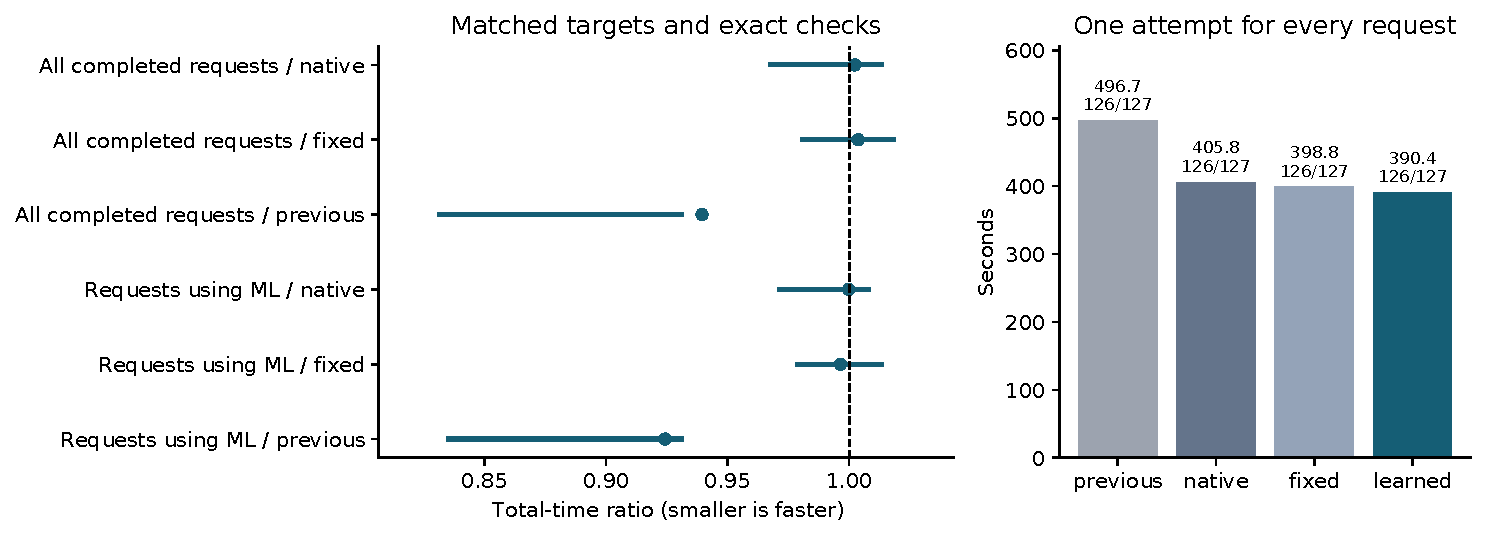
\includegraphics[width=\linewidth]{paper_figures/total_time_selection.pdf}
\caption{The left panel separates the complete application change from the added learned choice. Each point uses completed matched requests; bars show variation from resampling the three repetitions, and the dashed line marks equal time. The right panel includes one attempt for every requested calculation. Its labels give elapsed seconds and verified coverage, so an unfinished request cannot appear as a successful speedup.}
\label{fig:total-time}
\end{figure}
\begin{table}[!htbp]\centering\small
\caption{Use of the selector in each physical domain. The pentagon row is a subset of coupled requests. The ratio uses only matched requests that invoke the model, with the best fixed candidate as control. A dash means that no such comparison exists.}
\label{tab:total-domains}
\begin{tabularx}{\linewidth}{@{}Yrrrr@{}}\toprule
Domain & Requested & Verified & Use ML & ML/fixed\\\midrule
Coupled families & 49 & 48 & 31 & 0.988\\
Independent products & 52 & 52 & 51 & 0.999\\
Analytic formulas & 26 & 26 & 0 & --\\
Pentagon subset & 4 & 4 & 0 & --\\
\bottomrule\end{tabularx}\end{table}

Across every timed attempt, the learned application uses 1031.206 seconds, native choices use 1042.751, the fixed choice uses 1037.630, and the previous application uses 1207.572. These totals include all recorded repetitions and failures. Independent reference preparation takes 515.774 seconds outside the application timers. The existing checked master-basis preparation and training-label collection also precede deployment. The 497 training and validation action measurements use 1057.612 seconds in total, before independent reference preparation and 5.667 seconds of model fitting. The supplied-basis comparison therefore measures subsequent reductions, rather than a complete first-use calculation with unknown masters.

The high-loop results remain specific to the defined analytic families and products of small independent blocks. The coupled native tests reach three loops. No result establishes a globally minimum reduction time or complete coverage of arbitrary thirteen-loop scattering. The earlier seed and equation models retain their separate measured domains; the present selector keeps native equation and row choices, and we do not multiply savings from separate experiments.
